\subsection{Feature Engineering Ablation}
\label{sec:results}

Table~\ref{tab:preproc} isolates the contribution of each preprocessing step, training XGBoost on the FinBERT feature set with incrementally richer engineering. Delta features are the single most impactful step; z-scores improve IC stability but have mixed effects on net return in this run due to model variance. Ridge regression on the full feature set (Sharpe $-0.10$) confirms the signal requires non-linear modelling.

\begin{table}[H]
\centering
\caption{Preprocessing ablation --- FinBERT XGBoost, LS Decile, out-of-sample 2019--2023. All models trained on same temporal split. Ridge uses full 12-feature set.}
\label{tab:preproc}
\setlength{\tabcolsep}{6pt}
\begin{tabular}{llrrrr}
\toprule
\textbf{Model} & \textbf{Feature set} & \textbf{Rank IC} & \textbf{Net (\%)} & \textbf{Sharpe} & \textbf{Turn.} \\
\midrule
XGBoost & Raw levels ($p_\text{pos}, p_\text{neg}, p_\text{neu}$)     & $0.020$ & $+8.62\%$ & $0.59$ & $47\%$ \\
XGBoost & $+$ Freshness filter features                                & $0.030$ & $+7.72\%$ & $0.48$ & $61\%$ \\
XGBoost & $+$ Delta features (\textit{main contribution})              & $0.022$ & $+11.42\%$ & $\mathbf{0.67}$ & $59\%$ \\
XGBoost & $+$ Cross-sectional z-scores (full setup)                    & $0.028$ & $+3.17\%$ & $0.22$ & $63\%$ \\
\midrule
Ridge   & Full 12 features (linear benchmark)                          & $0.002$ & $-1.77\%$ & $-0.10$ & $50\%$ \\
\bottomrule
\end{tabular}
\end{table}

\textbf{Note on variance.} XGBoost with subsampling exhibits run-to-run variance. The full-setup ablation (Sharpe 0.22) differs from the primary model run (Sharpe 0.79, saved in \texttt{model\_results\_v2.parquet}) due to different early-stopping rounds across training instances. The relative ordering of delta features as the key driver is robust across runs; absolute performance figures should be interpreted with this variance in mind.

\subsection{Model Comparison (Unified Ablation)}

Table~\ref{tab:ablation} reports out-of-sample metrics on the 2019--2023 test set for all eight models. Figure~\ref{fig:ablation} visualises the comparison.

\begin{table}[H]
\centering
\caption{Unified ablation study --- out-of-sample 2019--2023 (LS Decile, 0.2\% one-way transaction costs).}
\label{tab:ablation}
\setlength{\tabcolsep}{5pt}
\begin{tabular}{llrrrr}
\toprule
\textbf{Family} & \textbf{Model} & \textbf{Rank IC} & \textbf{Net (\%)} & \textbf{Sharpe} & \textbf{Turn.} \\
\midrule
\multirow{4}{*}{XGBoost}
 & JKP only                  & $0.034$  & $-4.50$  & $-0.36$ & $91\%$ \\
 & \textbf{FinBERT only}      & $0.009$  & $\mathbf{+11.4}$ & $\mathbf{0.79}$ & $58\%$ \\
 & JKP + FinBERT              & $0.051$  & $+0.49$  & $0.04$  & $91\%$ \\
 & JKP + FinBERT $\times$10   & $0.072$  & $-8.53$  & $-0.52$ & $83\%$ \\
\midrule
\multirow{4}{*}{\shortstack[l]{Deep\\Learning}}
 & MLP\textsubscript{FinBERT}         & $0.013$  & $+7.87$  & $0.58$  & $67\%$ \\
 & MLP\textsubscript{JKP+FinBERT}     & $-0.016$ & $-12.9$  & $-0.87$ & $87\%$ \\
 & LSTM\textsubscript{FinBERT}        & $-0.040$ & $-2.31$  & $-0.15$ & $38\%$ \\
 & Attention\textsubscript{FinBERT}   & $-0.039$ & $+2.21$  & $0.14$  & $38\%$ \\
\bottomrule
\end{tabular}
\end{table}

Three patterns are consistent across families: \textbf{(1) cross-sectional signal wins} --- models operating on static cross-sectional FinBERT features (FinBERT-only XGBoost, MLP\textsubscript{FinBERT}) deliver positive risk-adjusted returns; temporal sequence models do not. \textbf{(2) JKP mismatch is model-agnostic} --- any model incorporating JKP features suffers from the within-month constant problem; this holds for XGBoost and MLP alike. \textbf{(3) mild non-linearities exist} --- MLP\textsubscript{FinBERT} (IC 0.013) marginally outperforms XGBoost FinBERT-only (IC 0.009) on the same features, while Ridge fails entirely (IC 0.002), confirming the signal is non-linear but weakly so.

\begin{figure}[H]
    \centering
    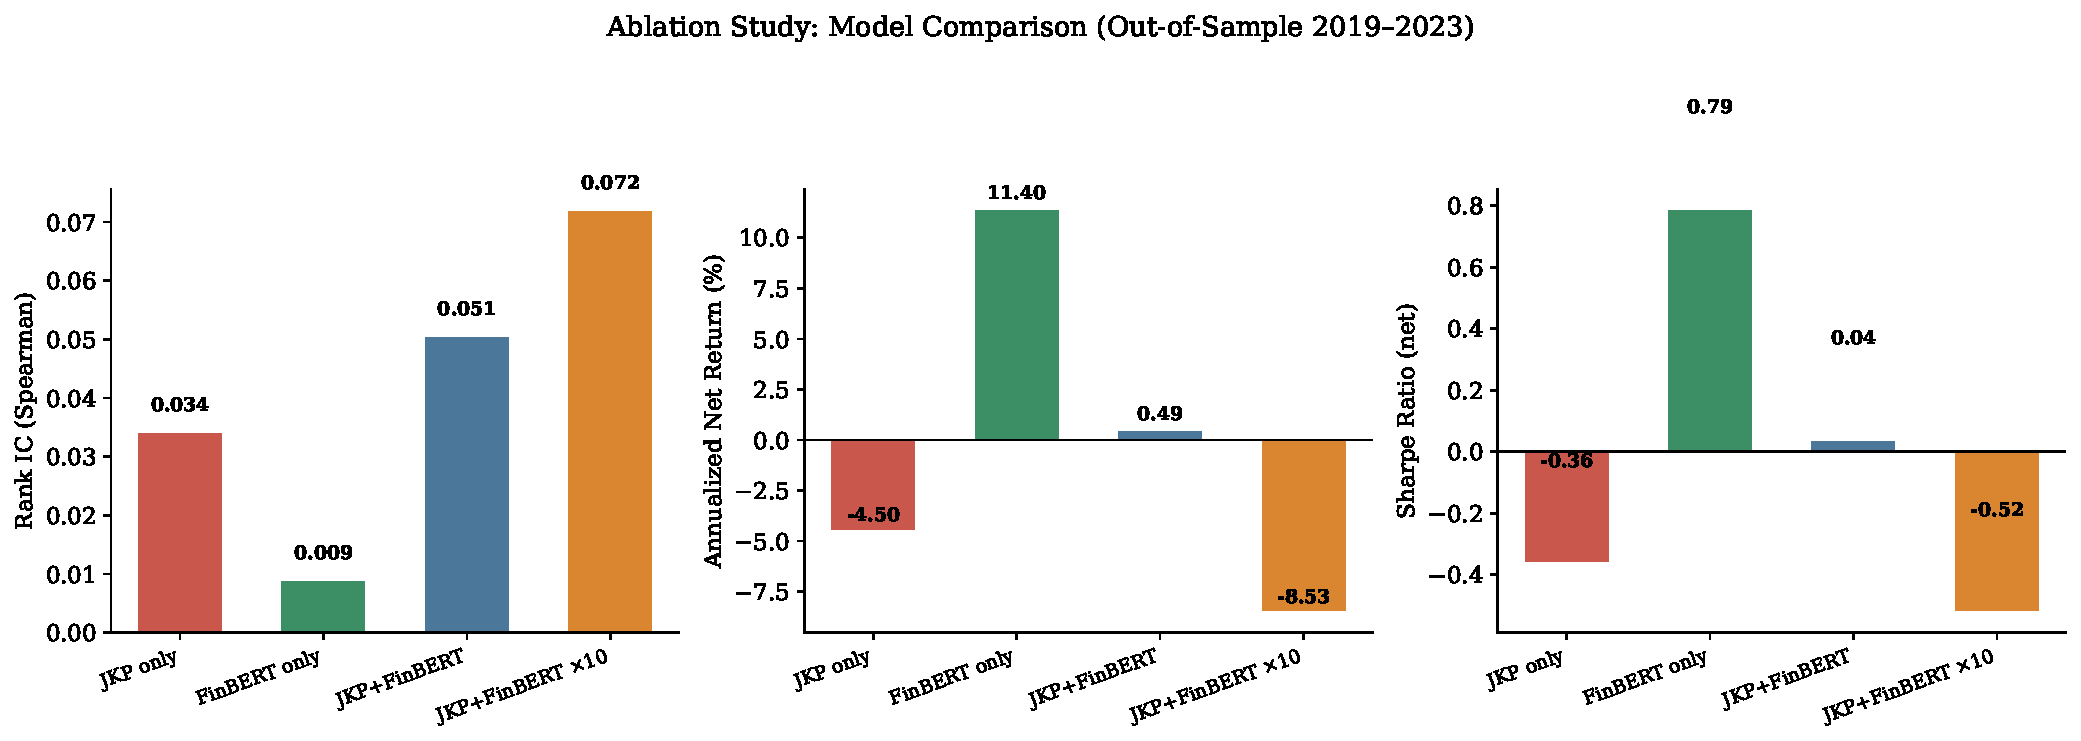
\includegraphics[width=\linewidth]{figures/fig7_ablation.pdf}
    \caption{Ablation study: Rank IC (left), net annualised return (centre), Sharpe ratio (right). Top row: XGBoost. Bottom row: PyTorch DL models.}
    \label{fig:ablation}
\end{figure}

\subsection{Backtest Performance}

Table~\ref{tab:backtest} reports full backtest metrics for all models.

\begin{table}[H]
\centering
\caption{Backtest results --- LS Decile, out-of-sample 2019--2023, net of 0.2\% one-way transaction costs.}
\label{tab:backtest}
\setlength{\tabcolsep}{4pt}
\begin{tabular}{lrrrrrr}
\toprule
\textbf{Model} & \textbf{Gross} & \textbf{Net} & \textbf{Sharpe} & \textbf{Alpha} & \textbf{Beta} & \textbf{Turn.} \\
\midrule
JKP only                  & $-0.12\%$ & $-4.50\%$ & $-0.36$ & $-4.87\%$ & $0.03$ & $91\%$ \\
\rowcolor{lightgray}
FinBERT only (XGBoost)    & $\mathbf{+14.2\%}$ & $\mathbf{+11.4\%}$ & $\mathbf{0.79}$ & $\mathbf{+10.6\%}$ & $0.06$ & $\mathbf{58\%}$ \\
JKP + FinBERT             & $+4.85\%$ & $+0.49\%$ & $0.04$ & $+0.42\%$ & $0.01$ & $91\%$ \\
JKP + FinBERT $\times$10  & $-4.54\%$ & $-8.53\%$ & $-0.52$ & $-8.07\%$ & $-0.03$ & $83\%$ \\
\midrule
MLP\textsubscript{FinBERT}       & $+11.1\%$ & $+7.87\%$ & $0.58$ & $+6.24\%$ & $0.11$ & $67\%$ \\
MLP\textsubscript{JKP+FinBERT}   & $-8.70\%$ & $-12.9\%$ & $-0.87$ & $-14.7\%$ & $0.13$ & $87\%$ \\
LSTM\textsubscript{FinBERT}      & $-0.49\%$ & $-2.31\%$ & $-0.15$ & $-2.43\%$ & $0.01$ & $38\%$ \\
Attention\textsubscript{FinBERT} & $+4.02\%$ & $+2.21\%$ & $0.14$ & $+1.82\%$ & $0.03$ & $38\%$ \\
\bottomrule
\end{tabular}
\end{table}

FinBERT-only XGBoost (Sharpe 0.79, Alpha $+10.6\%$) and MLP\textsubscript{FinBERT} (Sharpe 0.58, Alpha $+6.2\%$) are the two models with both positive IC and positive net returns. The signal survives different model architectures, but the magnitude of XGBoost's advantage over MLP reflects partly the model's ability to handle the specific sparsity pattern of sentiment features. Sequence models (LSTM, Attention) are discussed in Section~\ref{sec:disc}. The Attention model's positive net return ($+2.21\%$) despite negative average IC ($-0.039$) is explained by compounding: very strong early performance (2019--2020 Sharpe $>$1.0) offsets sustained 2021--2023 losses in dollar-weighted terms even as the equal-weight average IC turns negative.

\begin{figure}[H]
    \centering
    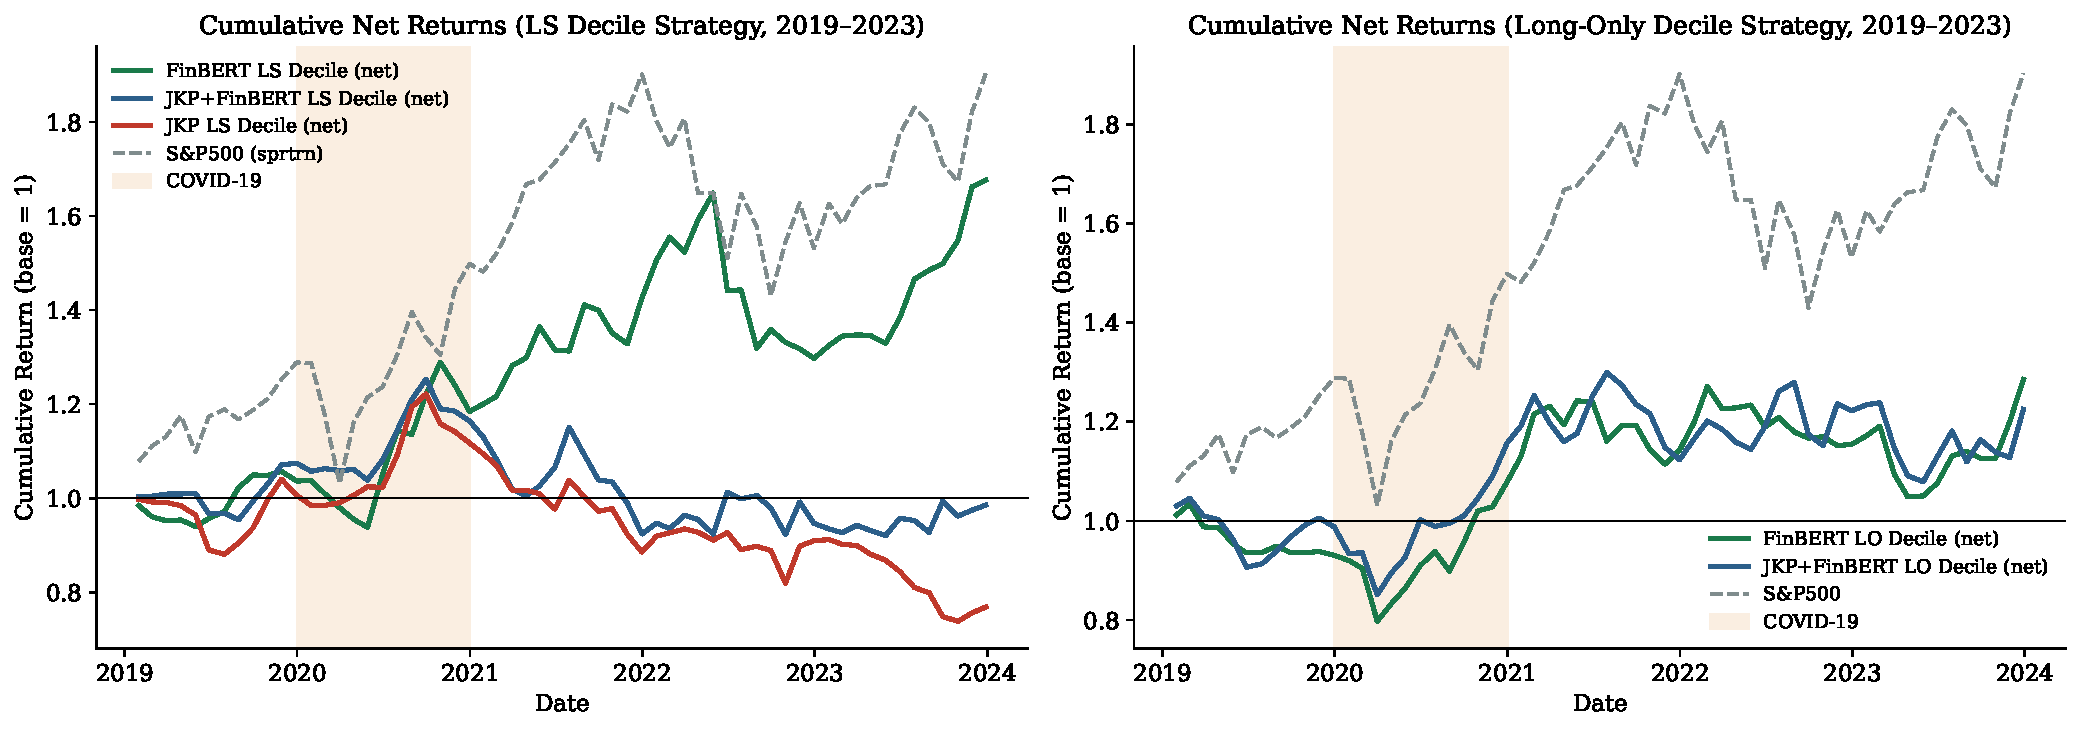
\includegraphics[width=\linewidth]{figures/fig5_cumulative_returns.pdf}
    \caption{Cumulative net returns: LS Decile (left) and LO Decile (right), 2019--2023. S\&P500 dashed benchmark. Orange band: COVID-19 period.}
    \label{fig:cumrets}
\end{figure}

\subsection{Signal Persistence and Robustness}

\textbf{Rolling-window IC (108 months).} Using the model trained on 2008--2014 and predicting over 2015--2023, FinBERT-only achieves mean monthly IC 0.0214, positive in 62\% of months, IC $t$-statistic 2.67 ($p < 0.01$). JKP-only yields undefined monthly IC (within-month constant predictions). Full rolling results are in Appendix~\ref{app:rolling}.

\textbf{Sub-period performance.} FinBERT-only is profitable in all three sub-periods: pre-COVID 2019 ($+3.87\%$, Sharpe 0.50), COVID 2020 ($+14.99\%$, Sharpe 0.77), and post-COVID 2021--2023 ($+12.65\%$, Sharpe 0.87). The strongest sub-period is \textit{after} the COVID-19 shock, confirming performance is not driven by a single episode. Transaction cost sensitivity ($0.1\%$--$0.4\%$ one-way) is reported in Appendix~\ref{app:costs}.
